% !BIB program = bibtex
% !TEX TS-program = xelatex
% !TeX spellcheck = ru_RU

\documentclass[13pt, russian]{matmex-diploma-custom}

% !TeX spellcheck = ru_RU
% !TEX root = vkr.tex
% Опциональные добавления используемых пакетов. Вполне может быть, что они вам не понадобятся, но в шаблоне приведены примеры их использования.
\usepackage{tikz} % Мощный пакет для создание рисунков, однако может очень сильно замедлять компиляцию
\usetikzlibrary{decorations.pathreplacing,calc,shapes,positioning,tikzmark}

% Библиотека для TikZ, которая генерирует отдельные файлы для каждого рисунка
% Позволяет ускорить компиляцию, однако имеет свои ограничения
% Например, ломает пример выделения кода в листинге из шаблона
% \usetikzlibrary{external}
% \tikzexternalize[prefix=figures/]

\newcounter{tmkcount}

\usepackage{fancyvrb} % для verbatim переноса строки

% --- переносы в коде/JSON ---
\usepackage{listings}
\lstset{
  basicstyle=\ttfamily\small,
  breaklines=true,           % перенос длинных строк
  breakatwhitespace=false,   % переносить можно в любом месте
  columns=fullflexible,      % корректная ширина моношрифта
  keepspaces=true,           % сохранять пробелы
  showstringspaces=false
}
% (необязательно) Определение простого языка JSON для подсветки
\lstdefinelanguage{json}{
  string=[s]{"}{"},
  morestring=[s]{'}{'}, % если вдруг одинарные кавычки
  comment=[l]{//},
}

\tikzset{
    use tikzmark/.style={
            remember picture,
            overlay,
            execute at end picture={
                    \stepcounter{tmkcount}
                },
        },
    tikzmark suffix={-\thetmkcount}
}

\usepackage{booktabs} % Пакет для верстки "более книжных" таблиц, вполне годится для оформления результатов
% В шаблоне есть команда \multirowcell, которой нужен этот пакет.
\usepackage{multirow}
\usepackage{siunitx} % для таблиц с единицами измерений

% Для названий стоит использовать \textsc{}
\newcommand{\OCaml}{\textsc{OCaml}}
\newcommand{\miniKanren}{\textsc{miniKanren}}
\newcommand{\BibTeX}{\textsc{BibTeX}}
\newcommand{\vsharp}{\textsc{V$\sharp$}}
\newcommand{\fsharp}{\textsc{F$\sharp$}}
\newcommand{\csharp}{\textsc{C\#}}
\newcommand{\GitHub}{\textsc{GitHub}}
\newcommand{\SMT}{\textsc{SMT}}

\definecolor{eclipseGreen}{RGB}{63,127,95}
% \lstdefinelanguage{ocaml}{
% keywords={@type, function, fun, let, in, match, with, when, class, type,
% nonrec, object, method, of, rec, repeat, until, while, not, do, done, as, val, inherit, and,
% new, module, sig, deriving, datatype, struct, if, then, else, open, private, virtual, include, success, failure,
% lazy, assert, true, false, end},
% sensitive=true,
% commentstyle=\small\itshape\ttfamily,
% keywordstyle=\ttfamily\bfseries, %\underbar,
% identifierstyle=\ttfamily,
% basewidth={0.5em,0.5em},
% columns=fixed,
% fontadjust=true,
% literate={->}{{$\to$}}3 {===}{{$\equiv$}}1 {=/=}{{$\not\equiv$}}1 {|>}{{$\triangleright$}}3 {\\/}{{$\vee$}}2 {/\\}{{$\wedge$}}2 {>=}{{$\ge$}}1 {<=}{{$\le$}} 1,
% morecomment=[s]{(*}{*)}
% }

\makeatletter
\@ifclassloaded{beamer}{
    %%% Обязательные пакеты
    %% Beamer
    \usepackage{beamerthemesplit}
    \usetheme{SPbGU}
    \beamertemplatenavigationsymbolsempty
    \usepackage{appendixnumberbeamer}

    %% Локализация
    \usepackage{fontspec}
    \setmainfont{CMU Serif}
    \setsansfont{CMU Sans Serif}
    \setmonofont{CMU Typewriter Text}
    %\setmonofont{Fira Code}[Contextuals=Alternate,Scale=0.9]
    %\setmonofont{Inconsolata}
    \usepackage{polyglossia}
    \setmainlanguage{russian}
    \setotherlanguage{english}

    %% Графика
    \usepackage{pdfpages} % Позволяет вставлять многостраничные pdf документы в текст

    % Математические окружения с русским названием
    \newtheorem{rutheorem}{Теорема}
    \newtheorem{ruproof}{Доказательство}
    \newtheorem{rudefinition}{Определение}
    \newtheorem{rulemma}{Лемма}
    \usepackage{fancyvrb}
}
{}
\makeatother

\usepackage[autostyle]{csquotes} % Правильные кавычки в зависимости от языка
\usepackage{totcount}
\usepackage{setspace}
\usepackage{amsmath, amsfonts, amssymb, amsthm, mathtools} % "Адекватная" работа с математикой в LaTeX



\begin{document}
% !TeX spellcheck = ru_RU
% !TEX root = vkr.tex

%% Если что-то забыли, при компиляции будут ошибки Undefined control sequence \my@title@<что забыли>@ru
%% Если англоязычная титульная страница не нужна, то ее можно просто удалить.
\filltitle{ru}{
    %% Актуально только для курсовых/практик. ВКР защищаются не на кафедре а в ГЭК по направлению,
    %%   и к моменту защиты вы будете уже не в группе.
    chair              = {Кафедра информатики},
    group              = {23.Б16-мм},
    %
    %% Макрос filltitle ненавидит пустые строки, поэтому обязателен хотя бы символ комментария на строке
    %% Актуально всем.
    title              = {Реализация и внедрение архитектуры Gated Recurrent Unit в пакет DEGANN},
    %
    %% Здесь указывается тип работы. Возможные значения:
    %%   production - производственная практика;
    %%   coursework - отчёт по курсовой работе (ОБРАТИТЕ ВНИМАНИЕ, у техпрога и ПИ нет курсовых, только практики);
    %%   practice - отчёт по учебной практике;
    %%   prediploma - отчёт по преддипломной практике;
    %%   master - ВКР магистра;
    %%   bachelor - ВКР бакалавра.
    type               = {practice},
    %
    %% Здесь указывается вид работы. От вида работы зависят критерии оценивания.
    %%   solution - «Решение». Обучающемуся поручили найти способ решения проблемы в области разработки программного обеспечения или теоретической информатики с учётом набора ограничений.
    %%   experiment - «Эксперимент». Обучающемуся поручили изучить возможности, достоинства и недостатки новой технологии, платформы, языка и т. д. на примере какой-то задачи.
    %%   production - «Производственное задание». Автору поручили реализовать потенциально полезное программное обеспечение.
    %%   comparison - «Сравнение». Обучающемуся поручили сравнить несколько существующих продуктов и/или подходов.
    %%   theoretical - «Теоретическое исследование». Автору поручили доказать какое-то утверждение, исследовать свойства алгоритма и т.п., при этом не требуя написания кода.
    kind               = {production},
    %
    author             = {Мурадян Денис Степанович},
    %
    %% Актуально только для ВКР. Указывается код и название направления подготовки. Типичные примеры:
    %%   02.03.03 \enquote{Математическое обеспечение и администрирование информационных систем}
    %%   02.04.03 \enquote{Математическое обеспечение и администрирование информационных систем}
    %%   09.03.04 \enquote{Программная инженерия}
    %%   09.04.04 \enquote{Программная инженерия}
    %% Те, что с 03 в середине --- бакалавриат, с 04 --- магистратура.
    specialty          = {02.03.03 \enquote{Математическое обеспечение и администрирование информационных систем}},
    %
    %% Актуально только для ВКР. Указывается шифр и название образовательной программы. Типичные примеры:
    %%   СВ.5162.2020 \enquote{Технологии программирования}
    %%   СВ.5080.2020 \enquote{Программная инженерия}
    %%   ВМ.5665.2022 \enquote{Математическое обеспечение и администрирование информационных систем}
    %%   ВМ.5666.2022 \enquote{Программная инженерия}
    %% Шифр и название программы можно посмотреть в учебном плане, по которому вы учитесь.
    %% СВ.* --- бакалавриат, ВМ.* --- магистратура. В конце --- год поступления (не обязательно ваш, если вы были в академе/вылетали).
    programme          = {СВ.5162.2020 \enquote{Технологии программирования}},
    %
    %% Актуально всем.
    %% Должно умещаться в одну строчку, допускается использование сокращений, но без переусердствования,
    %% короткая строка с большим количеством сокращений выглядит странно
    %supervisorPosition = {проф. кафeдры системного программирования, д.ф.-м.н.,}, % Терехов А. Н.
    %supervisorPosition = {ст. преподаватель кафедры ИАС, к.~ф.-м.~н. (если есть),}, % Смирнов К. К.
    supervisorPosition = {доцент кафедры системного программирования, к.ф.-м.н.,},
    supervisor         = {Гориховский~В.~И.},
    %
    %% Актуально только для практик и курсовых. Если консультанта нет или он совпадает с научником, закомментировать или удалить вовсе.
    consultantPosition = {Преподаватель СПбГУ,},
    consultant         = {Алимов~П.~Г.},
}

% Английский титульник нужен только для ВКР, остальные виды работ могут его смело игнорировать.
\filltitle{en}{
    chair              = {Advisor's chair},
    group              = {ХХ.BХХ-mm},
    title              = {Template for SPbU qualification works},
    type               = {bachelor},
    author             = {FirstName Surname},
    %
    %% Possible choices:
    %%   02.03.03 \foreignquote{english}{Software and Administration of Information Systems}
    %%   02.04.03 \foreignquote{english}{Software and Administration of Information Systems}
    %%   09.03.04 \foreignquote{english}{Software Engineering}
    %%   09.04.04 \foreignquote{english}{Software Engineering}
    %% Те, что с 03 в середине --- бакалавриат, с 04 --- магистратура.
    specialty          = {02.03.03 \foreignquote{english}{Software and Administration of Information Systems}},
    %
    %% Possible choices:
    %%   СВ.5162.2020 \foreignquote{english}{Programming Technologies}
    %%   СВ.5080.2020 \foreignquote{english}{Software Engineering}
    %%   ВМ.5665.2022 \foreignquote{english}{Software and Administration of Information Systems}
    %%   ВМ.5666.2022 \foreignquote{english}{Software Engineering}
    programme          = {СВ.5162.2020 \foreignquote{english}{Programming Technologies}},
    %
    %% Note that common title translations are:
    %%   кандидат наук --- C.Sc. (NOT Ph.D.)
    %%   доктор ... наук --- Sc.D.
    %%   доцент --- docent (NOT assistant/associate prof.)
    %%   профессор --- prof.
    supervisorPosition = {Sc.D, prof.},
    supervisor         = {S.S. Supervisor},
    %
    consultantPosition = {position at \foreignquote{english}{Company}, degree if present},
    consultant         = {C.C. Consultant},
    %
    reviewerPosition   = {position at \foreignquote{english}{Company}, degree if present},
    reviewer           = {R.R. Reviewer},
}

\maketitle
\setcounter{tocdepth}{2}
\tableofcontents

\newfontfamily\myfont{CMU Sans Serif}

% !TeX spellcheck = ru_RU
% !TEX root = vkr.tex

\section*{Введение}
\thispagestyle{withCompileDate}

Большинство людей в современном мире уже не представляет повседневную жизнь без больших языковых моделей (LLM). Они встроены в поисковые системы, офисные пакеты, средства разработки, клиентскую поддержку и образовательные платформы. Крупные компании используют LLM для улучшения пользовательского опыта, автоматизации рутины, повышения производительности и индивидуализации сервисов под конкретного клиента, что ускоряет внедрение интеллектуальных функций в бизнес-продукты.

Расширение сфер применения LLM неизбежно ведёт к расширению ответственности за их поведение, особенно в крупных экономических, политических и социально значимых проектах. Безопасность ответов модели, предсказуемость её поведения и устойчивость к злонамеренным воздействиям становятся критически важными требованиями. Ошибки, предвзятости или управляемые отклонения в поведении системы могут приводить к репутационным рискам, финансовым потерям и нарушению нормативных требований.

Одним из ключевых векторов атак на LLM являются \emph{промт-инъекции} - техники, с помощью которых злоумышленник подталкивает модель к нарушению исходных инструкций, политик или ожидаемых ограничений. В результате «дружелюбный помощник» может начать генерировать неуместные, грубые или вредоносные ответы, рекомендовать действия, противоречащие политике провайдера, либо выдавать информацию, распространение которой запрещено. Такие сценарии подрывают доверие к системам на базе LLM и повышают стоимость их сопровождения и контроля.

В данной работе мы систематически рассматриваем и исследуем разновидности промт-инъекций с точки зрения их вредоносности и возможных последствий для поведения модели. На основе этого исследования формируется и размечается корпус данных, предназначенный для разработки бенчмарка, который позволит комплексно тестировать различные модели и оценивать их устойчивость к инструкционным атакам.

% !TeX spellcheck = ru_RU
% !TEX root = vkr.tex

\section{Постановка задачи}
\label{sec:task}

Целью работы является расширение функциональности пакета DEGANN\cite{degann} --- путём внедрения рекуррентных нейронных сетей с архитектурой GRU (Gated Recurrent Unit)\cite{gru}.

Для её выполнения были поставлены следующие задачи:
\subsubsection{Общая архитектура решения}
\begin{enumerate}
    \item Реализация модуля с топологией рекуррентной сети со слоями tensorflow для архитектуры GRU и внедрение его в пакет DEGANN (раздел~\ref{subsec:topology});
    \item Создание модели с архитектурой GRU. Создание и интеграция callback-функции для расширения функциональности обучения и его трекинга (раздел~\ref{subsec:model_callbacks});
\end{enumerate}

\subsubsection*{Валидация решения}
\begin{enumerate}
    \item Создание датасета для корректной передачи данных в модель. Реализация сложно-аппроксимируемой функции для тестирования (раздел~\ref{subsec:dataset});
    \item Подбор метрики, настройка гиперпараметров (раздел~\ref{subsec:metrics});
\end{enumerate}

А так же обучить модель, продемонстрировать результаты в качестве сравнения значений лосс-функций и графиков аппроксимации.
% !TeX spellcheck = ru_RU
% !TEX root = vkr.tex

\section{Обзор}
\label{sec:relatedworks}

В данном разделе рассмотрены основные подходы и технологии, применяемые для извлечения данных с веб-страниц, а также существующие в литературе методы, близкие по назначению к задачам автоматизированного парсинга. Описаны их преимущества и недостатки с точки зрения универсальности, надёжности и затрат вычислительных ресурсов.

\subsection{Методы парсинга веб-страниц}

Существует два классических метода парсинга веб-страниц: \emph{статический} и \emph{динамический}.

\paragraph{Статический парсинг} предполагает получение HTML-исходников напрямую через HTTP-запросы. Данный подход широко используется благодаря простоте реализации и высокой скорости работы. Типовой стек включает:
\begin{itemize}
    \item \textbf{Requests} — библиотека для отправки HTTP-запросов (документация Python\cite{python-official}).
    \item \textbf{BeautifulSoup4}\cite{bs4-doc} — парсер HTML/XML, позволяющий строить дерево тегов, искать элементы по селекторам и извлекать текст. Этот метод эффективен для страниц, контент которых формируется на сервере, но не подходит для SPA.
\end{itemize}
Преимущества статического подхода:
\begin{itemize}
    \item высокая производительность (ограничивается временем сетевых запросов и обработкой текста);
    \item простота отладки и воспроизводимость результатов при неизменном HTML.
\end{itemize}
Недостатки:
\begin{itemize}
    \item неспособность корректно обрабатывать страницы с интенсивным JavaScript;
    \item необходимость ручного написания селекторов для каждой новой страницы.
\end{itemize}

\paragraph{Динамический парсинг} предполагает эмуляцию браузера и выполнение JavaScript для получения «отрендеренного» DOM. К популярным инструментам относится:
\begin{itemize}
    \item \textbf{Selenium}\cite{selenium-doc} — фреймворк для автоматизации браузера, позволяющий запускать Chrome/Firefox в фоновом режиме, ждать загрузки страницы и затем извлекать итоговый HTML. Такой метод подходит для современных SPA, но более медленный и ресурсоёмкий по сравнению со статическим парсингом.
\end{itemize}
Преимущества:
\begin{itemize}
    \item возможность корректной обработки JavaScript-контента;
    \item высокая точность извлечения данных с динамических страниц.
\end{itemize}
Недостатки:
\begin{itemize}
    \item значительные накладные расходы на запуск браузера и ожидание рендеринга;
    \item зависимость от версий браузерных движков и драйверов.
\end{itemize}

\paragraph{Подходы на основе языковых моделей (LLM)} приобрели популярность после публикации работы Brown et al.\cite{brown2020language}, где продемонстрированы возможности LLM в «few-shot» режиме. В контексте парсинга LLM применяются в двух основных режимах:
\begin{itemize}
    \item \emph{Структурирование} (structuring) — LLM получает на вход очищенный HTML и текстовое описание необходимых полей, после чего возвращает готовую JSON-структуру. Этот метод снимает необходимость ручного написания селекторов, но многократные запросы к LLM могут быть дорогостоящими и медленными.
    \item \emph{Генерация кода} (codegen) — LLM формирует фрагмент Python-скрипта, который затем выполняется локально для извлечения данных. Такой подход сочетает гибкость LLM и возможность дальнейшей повторной работы без дополнительных запросов к модели.
\end{itemize}
Преимущества LLM-подходов:
\begin{itemize}
    \item высокая адаптивность к разнообразным HTML-структурам;
    \item возможность «понимания» семантики страницы без явного знания её DOM-структуры.
\end{itemize}
Недостатки:
\begin{itemize}
    \item необходимость вычислительных ресурсов и ограничение по числу токенов при обращении к облачным API;
    \item задержки при получении ответа от модели (latency);
    \item нестабильность результатов в «zero-shot» условиях.
\end{itemize}

\subsection{Используемые технологии}

Ниже приведён перечень ключевых технологий, используемых для реализации системы парсинга.

\paragraph{Язык программирования}
\begin{itemize}
    \item \textbf{Python}\cite{python-official} — выбран за счёт развитой экосистемы для веб-разработки, парсинга HTML и взаимодействия с LLM, а также встроенной поддержки SQLite.
\end{itemize}

\paragraph{HTTP-запросы и статический парсинг}
\begin{itemize}
    \item \textbf{Requests} (через\cite{python-official}) — инструмент для отправки HTTP-запросов в Python.
    \item \textbf{BeautifulSoup4}\cite{bs4-doc} — библиотека для парсинга HTML и XML.
\end{itemize}

\paragraph{Динамический парсинг}
\begin{itemize}
    \item \textbf{Selenium}\cite{selenium-doc} — фреймворк для автоматизации браузера, позволяющий получать «отрендеренный» HTML.
\end{itemize}

\paragraph{LLM-интеграция}
\begin{itemize}
    \item \textbf{MistralAI (mistralai Python SDK)}\cite{mistral-github} — клиентская библиотека для работы с LLM Mistral.
    \item \textbf{tiktoken}\cite{tiktoken-github} — утилита для подсчёта токенов, оптимизирующая стоимость запросов к LLM.
    \item \textbf{Brown et al.\cite{brown2020language}} — базовая статья, демонстрирующая потенциал LLM в режиме «few-shot».
\end{itemize}

\paragraph{Хранение кэша}
\begin{itemize}
    \item \textbf{SQLite (\texttt{sqlite3})}\cite{sqlite-official} — встраиваемая SQL-база для хранения метаданных и кэшированных скриптов.
\end{itemize}

\paragraph{Пользовательские интерфейсы}
\begin{itemize}
    \item \textbf{FastAPI}\cite{fastapi-official} — фреймворк для разработки REST-API.
    \item \textbf{Gradio}\cite{gradio-official} — библиотека для быстрой разработки веб-интерфейсов, развёртываемых в Hugging Face Space.
    \item \textbf{Jinja2}\cite{jinja2-official} — шаблонизатор для генерации HTML-страниц в веб-приложении.
\end{itemize}

\subsection{Выводы}

Из анализа существующих решений следует, что статический парсинг (Requests + BeautifulSoup4) эффективен для простых HTML-страниц, но не справляется с динамическими приложениями, требующими JavaScript (Selenium). Применение LLM (см.\cite{brown2020language}) открывает новые возможности автоматизации, однако требует значительных ресурсов и времени. Для создания универсального решения оправдан комбинированный подход, сочетающий традиционные методы парсинга с LLM-интеграцией и кэшированием, что позволяет оптимизировать вычислительные расходы и обеспечить повторный доступ к ранее сгенерированным парсер-скриптам.

% !TeX spellcheck = ru_RU
% !TEX root = vkr.tex

\section{Описание решения}

Перед тем как подробно рассмотреть реализацию, приведём схематичный алгоритм работы системы:
\begin{enumerate}
    \item Получение веб-страницы: определение необходимости JS-рендеринга с помощью \texttt{is\_dynamic\_site(url, timeout)} (см.\cite{PatilWebScraping2021, Smith2022}) и загрузка содержимого (статический запрос \cite{RequestsDocumentation} или рендеринг через Selenium \cite{SeleniumDocumentation}).
    \item Очистка HTML: выбор стратегии очистки (\texttt{FullCleaningStrategy} или \texttt{LightCleaningStrategy} \cite{Richardson2013, Brown2020}) в зависимости от режима (\emph{Structuring} или \emph{Codegen}).
    \item Интеграция с LLM: формирование промптов и вызов \texttt{LLMClient} из библиотеки MistralAI \cite{MistralAIDocumentation}, генерация структурированных данных (Structuring) или кода-парсера (Codegen) \cite{Kalyan2023, Li2024}.
    \item Кэширование: сохранение сгенерированных скриптов и/или результатов структурирования в SQLite и ChromaDB \cite{SQLiteDocumentation, ChromaDBDocumentation, Reimers2019} для повторного использования без дополнительных обращений к LLM \cite{Dong2022CacheLLM}.
    \item Выполнение парсера или разбора JSON: если найден кэш, загружается готовый скрипт; иначе выполняется вновь сгенерированный код или парсинг через Structuring, результат возвращается в формате JSON.
    \item Вывод результата пользователю через Gradio, REST-API или веб-frontend \cite{FastAPIDocumentation, GradioDocumentation, Jinja2Documentation}.
\end{enumerate}

В проекте реализованы два основных режима работы с LLM:
\begin{itemize}
    \item \emph{Structuring} — прямая генерация структурированных данных (JSON) из текста страницы \cite{Brown2020}.
    \item \emph{Codegen} — генерация Python-скрипта-парсера, который затем выполняется локально \cite{Dong2022CacheLLM}.
\end{itemize}
Для уменьшения затрат на повторные обращения к LLM внедрён механизм кэширования, использующий как реляционную базу SQLite, так и векторную базу ChromaDB для семантического поиска близких запросов \cite{Reimers2019, ChromaDBDocumentation}.

\subsection{Получение и предварительная обработка веб-страницы}
\label{subsec:solution1}

Чтобы определить, требуется ли JavaScript-рендеринг, используется функция \texttt{is\_dynamic\_site(url, timeout)} (файл \texttt{autoparse/tools/fetchers/dynamic\_detector.py}). Она возвращает \texttt{True}, если хотя бы один из следующих критериев выполнен:
\begin{enumerate}
    \item Статический HTTP-запрос (\texttt{fetch\_static\_html(url, timeout)}) завершился ошибкой \cite{RequestsDocumentation}.
    \item После парсинга через BeautifulSoup длина текста внутри тега \texttt{<body>} менее 300 символов \cite{Richardson2013}.
    \item В документе более 10 тегов \texttt{<script>}.
    \item У любого тега \texttt{<script>} атрибут \texttt{type} равен \texttt{"module"} или \texttt{"application/json"}.
    \item В атрибуте \texttt{src} тега \texttt{<script>} встречаются подстроки \texttt{"react", "angular", "vue", "ember", "svelte", "next", "nuxt"} \cite{W3Techs2024}.
    \item Содержимое inline-скриптов содержит \texttt{"window.\_\_"} или \texttt{"hydrate("}.
    \item В DOM присутствуют атрибуты гидрации: \texttt{data-reactroot}, \texttt{data-reactid}, \texttt{data-vue} или \texttt{data-server-rendered}.
    \item В документе найден элемент с \texttt{id} равным одному из \texttt{"app", "root", "main", "container", "next", "nuxt"}.
\end{enumerate}

В классе \texttt{Parser} (\texttt{autoparse/parser.py}) метод \texttt{parse\_url(url, \dots)} действует так:
\begin{itemize}
    \item Если \texttt{dynamic=True} или \texttt{is\_dynamic\_site(url)} возвращает \texttt{True}, вызывается рендеринг через Selenium (Headless Chrome) \cite{SeleniumDocumentation}.
    \item Иначе применяется статический HTTP-запрос через \texttt{requests} \cite{RequestsDocumentation}.
\end{itemize}
Далее полученный HTML передаётся на этап очистки (см. раздел~\ref{subsec:solution2}).

\subsection{Стратегии очистки HTML-разметки}
\label{subsec:solution2}

Для подготовки HTML к работе с LLM определены две стратегии (интерфейс \texttt{CleaningStrategy} в \texttt{autoparse/strategies/cleaning.py}):

\paragraph{FullCleaningStrategy.}
Полностью удаляет все HTML-теги и возвращает «чистый» текст. Применяется в режиме \emph{Structuring}, когда модель должна «прочитать» текст страницы и сформировать JSON-структуру \cite{Brown2020}. Алгоритм:
\begin{itemize}
    \item Удаление тегов \texttt{<script>}, \texttt{<style>} и комментариев.
    \item Сбор оставшегося текста через метод \texttt{BeautifulSoup.get\_text()} \cite{BeautifulSoupDocumentation}.
\end{itemize}

\paragraph{LightCleaningStrategy.}
Сохраняет базовую структуру HTML, удаляя лишь шумовые элементы (скрипты, стили, комментарии). Применяется в режиме \emph{Codegen}, когда LLM должно получить «облегчённый» HTML для генерации кода-парсера \cite{Dong2022CacheLLM}. Алгоритм:
\begin{itemize}
    \item Удаление тегов \texttt{<script>} и \texttt{<style>}.
    \item Удаление комментариев.
    \item Возврат оставшегося HTML-содержимого.
\end{itemize}

\paragraph{Диспетчер стратегий.}
Метод \texttt{get\_pipeline(html, mode, code\_cache)} (\texttt{autoparse/dispatcher.py}) возвращает пару «стратегия очистки + стратегия парсинга»:
\begin{itemize}
    \item \texttt{mode == "structuring"}: \texttt{FullCleaningStrategy} и \texttt{StructuringParsingStrategy}.
    \item \texttt{mode == "codegen"}: \texttt{LightCleaningStrategy} и \texttt{CodegenParsingStrategy}.
    \item \texttt{mode == "auto"}: если \texttt{is\_dynamic\_site(url)} → как для \emph{Structuring}, иначе → как для \emph{Codegen}.
\end{itemize}

\subsection{Интеграция с LLM: режимы \emph{Structuring} и \emph{Codegen}}
\label{subsec:solution3}

Работа с LLM реализована в папке \texttt{autoparse/tools/llm}. Ниже приведены текстовые описания основных компонентов и алгоритмов.

\subsubsection{Клиент LLM: \texttt{LLMClient}}
\label{sssec:llmclient}

Класс \texttt{LLMClient} (файл \texttt{client.py}) оборачивает SDK MistralAI \cite{MistralAIDocumentation}. Основные моменты:
\begin{itemize}
    \item При инициализации получает API-ключ (\texttt{MISTRAL\_API\_KEY}) и имя модели (\texttt{LLM\_MODEL="mistral-large-latest"}).
    \item Метод \texttt{call\_llm(prompt: str)} отправляет текстовый \texttt{prompt} и возвращает ответ модели в виде строки.
    \item Учитываются ограничения по лимиту токенов через \texttt{tiktoken} \cite{TiktokenDocumentation}.
\end{itemize}

\subsubsection{Режим \emph{Structuring}}
\label{sssec:structuring}

Алгоритм \texttt{StructuringParsingStrategy} выполняется так:
\begin{enumerate}
    \item На вход подаётся «чистый» текст (результат \texttt{FullCleaningStrategy}) и пользовательский запрос (\texttt{user\_query}).
    \item Формируется системный prompt с описанием задачи («Produce JSON…» \cite{Brown2020}) и вставляется сам текст страницы вместе с запросом.
    \item Вызывается \texttt{LLMClient.call\_llm(prompt)}, получаем ответную строку в формате JSON.
    \item Результат обрабатывается через \texttt{json.loads(response\_text)} и возвращается в виде словаря (\texttt{\{"structured\_data": <данные>\}}).
\end{enumerate}

\subsubsection{Режим \emph{Codegen}}
\label{sssec:codegen}

В режиме \emph{Codegen} применяется \texttt{LightCleaningStrategy} и компонент \texttt{hintgen}, который формирует контекст для генерации кода-парсера \cite{Li2024}. Ключевые шаги:
\begin{enumerate}
    \item \textbf{Получение «облегчённого» HTML.} Применяется \texttt{LightCleaningStrategy}, полученный HTML передаётся дальше.
    \item \textbf{Генерация подсказки (\texttt{hintgen}).} Модуль анализирует очищенный HTML и учёт запроса (\texttt{user\_query}), рассчитывает количество токенов через \texttt{tiktoken}, обрезает контекст и формирует Chat-style prompt, включающий:
    \begin{itemize}
        \item Системную инструкцию, объясняющую, какие теги и селекторы искать.
        \item Примеры полей и формат вывода.
        \item Собственно «облегчённый» HTML-фрагмент и запрос пользователя.
    \end{itemize}
    \item \textbf{Поиск в кэше (\texttt{ParserCodeCache.find\_similar}).}
    \begin{itemize}
        \item Формируется уникальный идентификатор \texttt{doc\_id = f"{url}:{user\_query}"}, вычисляется его embedding через модель \texttt{paraphrase-multilingual-MiniLM-L12-v2} \cite{Reimers2019}.
        \item Выполняется запрос к ChromaDB: если косинусное сходство ≥ порога (\texttt{SIMILARITY\_THRESHOLD}), возвращается путь к ранее сгенерированному скрипту из SQLite (кэш считается «попавшим»).
    \end{itemize}
    \item \textbf{Сохранение нового скрипта (если кэш не найден).}
    \begin{itemize}
        \item Вычисляется MD5-хеш от \texttt{url + user\_query}, формируется имя файла \texttt{<hash>.py} в папке \texttt{parsers/}.
        \item Полученный код записывается в этот файл, и в SQLite добавляется новая запись с полями \texttt{url, user\_query, file\_path, timestamp} \cite{SQLiteDocumentation}.
        \item Вычисляется embedding для \texttt{doc\_id} и добавляется в ChromaDB вместе с метаданными (время создания) \cite{ChromaDBDocumentation}.
    \end{itemize}
    \item \textbf{Возврат результата.} Если найден существующий файл, сразу возвращается готовый скрипт; иначе возвращается вновь сгенерированный код в формате JSON вида \texttt{\{"parser\_code": "<python\_code>"\}}.
\end{enumerate}

Таким образом, при наличии «эквивалентного» скрипта пара (\texttt{url}, \texttt{user\_query}) обрабатывается без повторного обращения к LLM, что позволяет снизить затраты и уменьшить задержки \cite{Dong2022CacheLLM, OpenAI2023Costs}.

\subsection{Механизм кэширования и семантического поиска запросов}
\label{subsec:solution4}

Класс \texttt{ParserCodeCache} (\texttt{autoparse/cache/code\_cache.py}) отвечает за хранение и поиск ранее созданных скриптов. Основные моменты:

\paragraph{Инициализация SQLite и ChromaDB.}
При создании \texttt{ParserCodeCache(base\_dir)}:
\begin{itemize}
    \item Создаётся папка \texttt{<base\_dir>/parsers/} для хранения Python-файлов.
    \item Открывается (или создаётся) файл \texttt{<base\_dir>/cache.db}.
    \item Выполняется SQL-команда, создающая таблицу \texttt{code\_cache} с полями \texttt{url}, \texttt{user\_query}, \texttt{file\_path} и \texttt{timestamp}, а также первичным ключом (\texttt{url, user\_query}) \cite{SQLiteDocumentation}.
    \item Инициализируется клиент ChromaDB и embedding-функция (Sentence-BERT), после чего из SQLite загружаются все имеющиеся записи: для каждой записи вычисляется embedding идентификатора \texttt{url:user\_query} и добавляется в коллекцию ChromaDB \cite{Reimers2019, ChromaDBDocumentation}.
\end{itemize}

\paragraph{Поиск «похожих» запросов.}
Метод \texttt{find\_similar(url, user\_query)}:
\begin{enumerate}
    \item Формирует \texttt{doc\_id = f"{url}:{user\_query}"} и вычисляет embedding через модель SentenceTransformer \cite{Reimers2019}.
    \item Делает запрос к коллекции ChromaDB, запрашивая ближайшего соседа. Если его косинусное сходство >= порога (\texttt{SIMILARITY\_THRESHOLD}), извлекает путь к файлу из SQLite и возвращает его; иначе возвращает \texttt{None}.
\end{enumerate}

\paragraph{Сохранение нового скрипта.}
Если \texttt{find\_similar} вернул \texttt{None}, производится:
\begin{enumerate}
    \item Генерация MD5-хеша от строки \texttt{url + user\_query}, формирование имени файла \texttt{<hash>.py} в директории \texttt{parsers/} \cite{Dong2022CacheLLM}.
    \item Запись полученного кода в файл.
    \item Вставка новой записи в таблицу \texttt{code\_cache} (через SQL-команду \texttt{INSERT OR IGNORE} с параметрами \texttt{url, user\_query, file\_path, timestamp}) \cite{SQLiteDocumentation}.
    \item Вычисление embedding для \texttt{doc\_id} и добавление его вместе с путём к файлу в коллекцию ChromaDB \cite{ChromaDBDocumentation}.
\end{enumerate}

\subsection{Пользовательские интерфейсы}
\label{subsec:solution5}

Для удобства взаимодействия с системой созданы три клиента, все они используют единый фасад: функцию \texttt{run\_agent} из модуля \texttt{agent/agent.py}. Ниже приводятся краткие описания.

\subsubsection{Gradio-приложение (Hugging Face Space)}

В файле \texttt{server/HFspace/app.py} настроен интерфейс на основе Gradio, который содержит:
\begin{itemize}
    \item Поле для ввода URL.
    \item Поле для ввода \texttt{user\_query}.
    \item Радиокнопки для выбора режима (\texttt{"auto", "structuring", "codegen"}).
    \item Флаг \texttt{dynamic} для принудительного указания необходимости рендеринга.
    \item Кнопка «Submit», вызывающая функцию вида:
    \begin{quote}
      \texttt{parse\_interface(url, query, mode, dynamic) = run\_agent(\dots)}
    \end{quote}
    Полученный результат (JSON или код-парсер) автоматически отображается через Gradio \cite{GradioDocumentation}.
\end{itemize}

\subsubsection{REST-API на FastAPI}

В файле \texttt{server/api/main.py} реализовано:
\begin{itemize}
    \item Pydantic-модель \texttt{ParseRequest} с полями \texttt{url, user\_query, mode, dynamic}.
    \item POST-эндпоинт \texttt{/parse}, который принимает JSON-запрос, вызывает \texttt{run\_agent} и возвращает ответ в формате JSON.
    \item Для запуска сервера используется команда:
    \begin{quote}
      \texttt{uvicorn server.api.main:app --reload}
    \end{quote}
    \cite{FastAPIDocumentation}.
\end{itemize}

\subsubsection{Веб-frontend (FastAPI + Jinja2 + JavaScript)}

\begin{figure}[h]
    \centering
    \begin{minipage}[b]{0.48\textwidth}
        \centering
        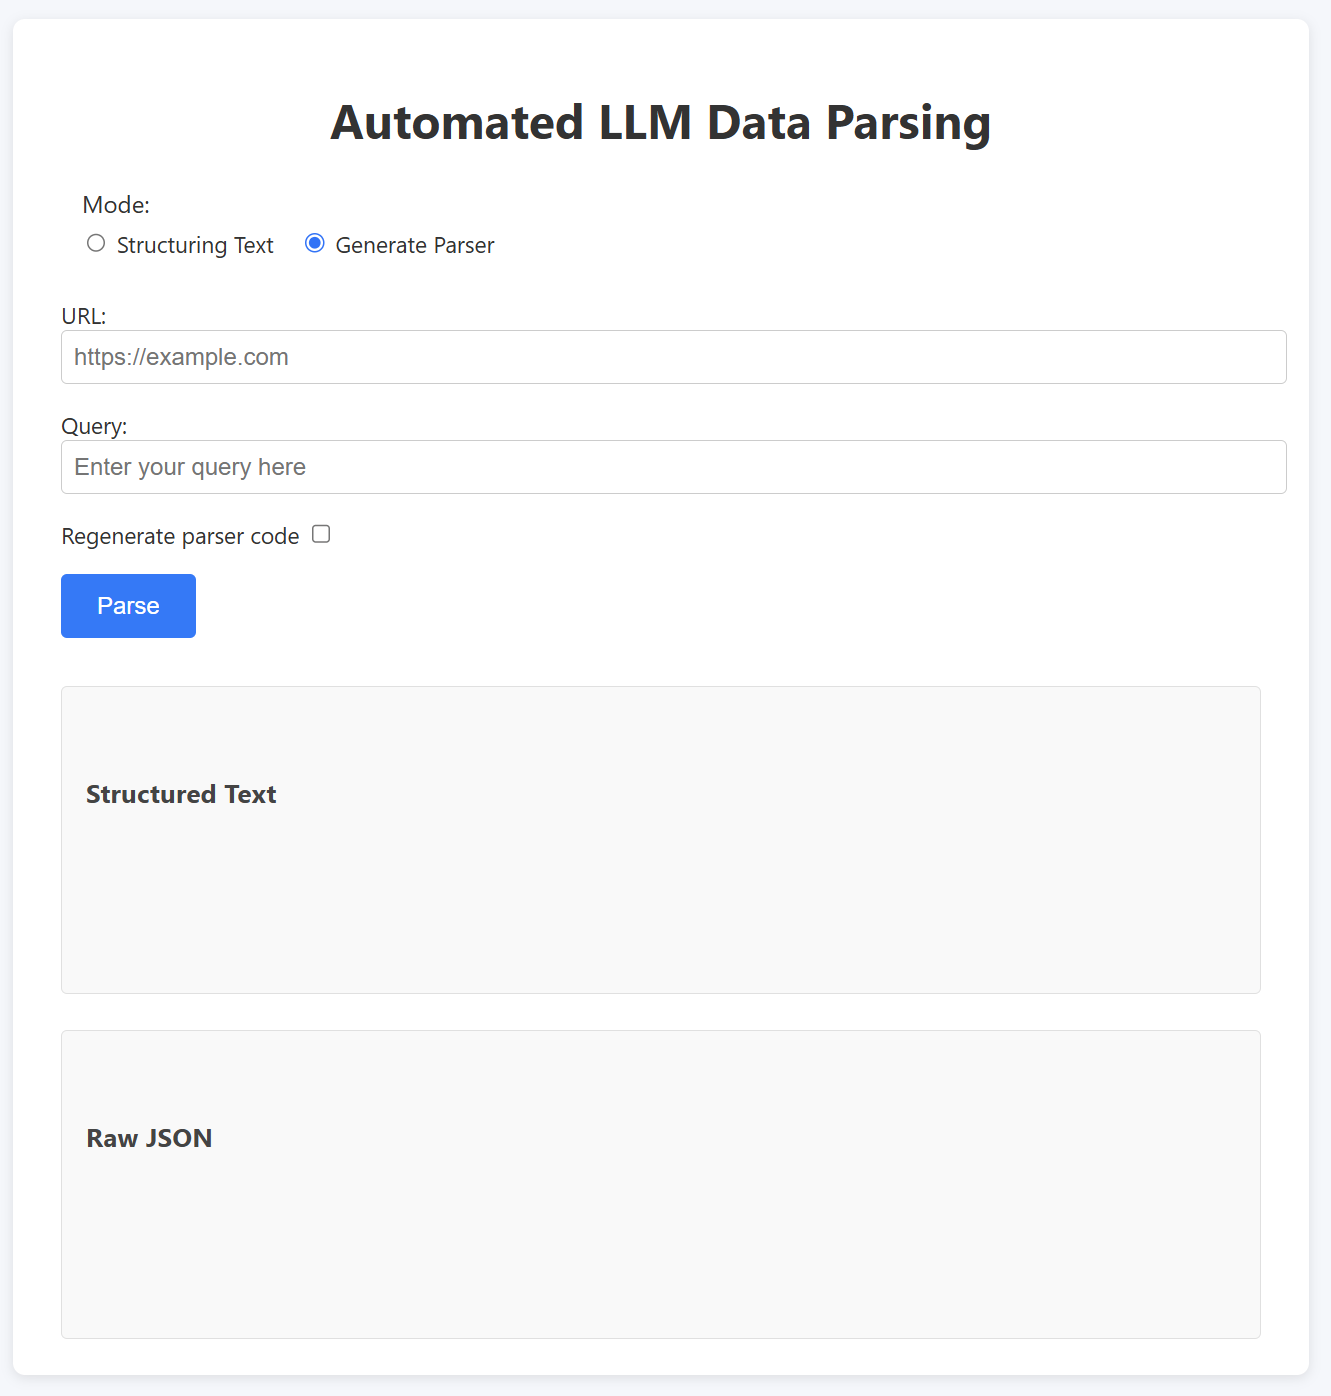
\includegraphics[width=\textwidth]{Include/dashboard_codegen.png}
        \caption{Веб-frontend: режим Codegen}
        \label{fig:dash_codegen}
    \end{minipage}
    \hfill
    \begin{minipage}[b]{0.48\textwidth}
        \centering
        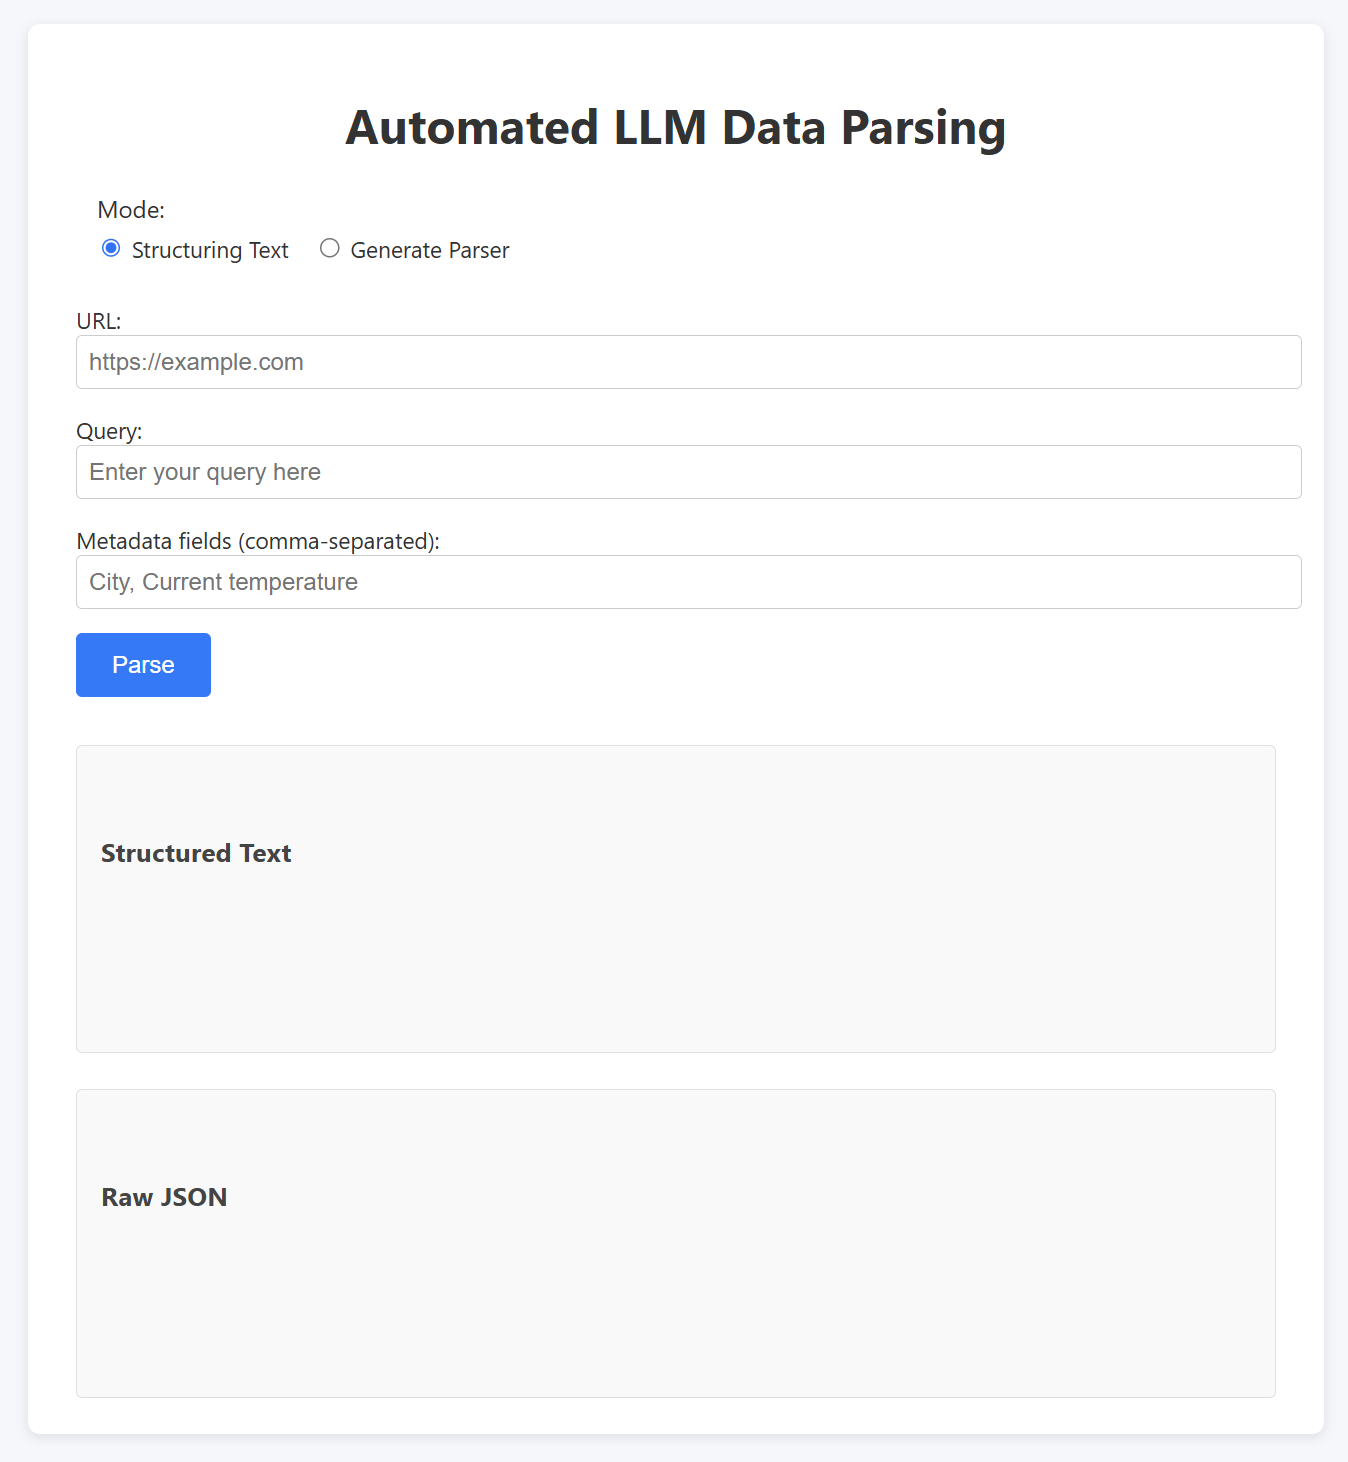
\includegraphics[width=\textwidth]{Include/dashboard_structuring.png}
        \caption{Веб-frontend: режим Structuring}
        \label{fig:dash_structuring}
    \end{minipage}
\end{figure}

В директории \texttt{server/web} настроено:
\begin{itemize}
    \item \texttt{main.py}, который монтирует статические файлы и рендерит шаблон \texttt{index.html}.
    \item В \texttt{templates/index.html} размещена HTML-форма с полями для URL, \texttt{user\_query}, выбора режима и флажка \texttt{dynamic}.
    \item JavaScript-файл \texttt{static/js/app.js} перехватывает отправку формы, выполняет AJAX-запрос к эндпоинту \texttt{/parse\_via\_web} и отображает полученный JSON или код в элементе \texttt{<div id="result">} \cite{Jinja2Documentation}.
\end{itemize}
%\section{Эксперимент}
%\label{subsec:results}

%% !TeX spellcheck = ru_RU
%% !TEX root = vkr.tex
%
%\section{Заключение}

%% !TeX spellcheck = ru_RU
%% !TEX root = vkr.tex
%
%\appendix
%\section{Приложение}


\setmonofont{CMU Typewriter Text}
\bibliographystyle{ugost2008ls}
\bibliography{vkr}

\end{document}
